\chapter*{Ejercicios del capítulo 1}
\addcontentsline{toc}{chapter}{Hoja 1}
\section*{Ejercicio 1}
\begin{mybox}
    Una nave despega de la Tierra el 1 de enero de 2050 y viaja durante 5
    años según el calendario de a bordo con una aceleración $g$ también medida
    con los instrumentos de a bordo. Luego desacelera al mismo ritmo durante
    otros 5 años, da media vuelta y regresa de idéntica manera. ¿Cual es la fecha
    de llegada en la Tierra? ¿A qué distancia llegó la nave?
\end{mybox}
Qué sabemos: asumiendo que $g>0$...\\
¿El sistema de referencia propio \emph{no} es inercial?
\begin{itemize}
    \item Los instrumentos de medida de la nave miden una aceleración $g$, alejándonos de la Tierra, con respecto a nuestro tiempo propio. Es decir, vemos cómo la Tierra se  ``aleja``  con aceleración $g$. La velocidad relativa, $v$, entre la nave y la Tierra \emph{con respecto a nuestro tiempo propio} es:
    $$
    v(\tau) = v_0 \pm g\tau 
    $$
    para los cuatro tramos del viaje. En función de en qué sentido se mueva la nave o si acelera o disminuye, tendremos una expresión de la velocidad distinta. 
\end{itemize}
Lo mejor será calcular el tiempo transcurrido en la Tierra para esa velocidad genérica, y luego especificar para cada tramo. En ese caso, según la ley de dilatación temporal,
\begin{equation*}
\begin{split}
    \D{t} = \gamma (v) \D{\tau} \implies \Delta t &= \int_{\tau_0}^{\tau_1} \D{\tau} \cdot \gamma (\tau) = \int_{\tau_0}^{\tau_1} \frac{\D{\tau}}{\sqrt{1-\beta (\tau)^2}} = \pm \frac{c}{g} \int_{\tau_0}^{\tau_1}  \frac{\D{\tau}\cdot \dot{\beta }}{\sqrt{1-\beta ^2}} \\
    &= \left .\pm \frac{c}{g} \arcsin \beta (v) \right |_{\tau_0}^{\tau_1} = \left .\pm \frac{c}{g} \arcsin \left (\frac{v_0\pm g\tau}{c} \right ) \right |_{\tau_0}^{\tau_1}
\end{split}
\end{equation*}
Ahora especificamos:
\begin{itemize}
    \item Para $0\le \tau \le 5$ años: $v = g\tau $.
    $$
    \Delta t = \left . \frac{c}{g}\arcsin \left (\frac{g}{c}\tau \right ) \right |_{0}^{5} = \boxed{\frac{c}{g}\arcsin\left ( \frac{5g}{c} \right )}
    $$

    \item Para $5\le \tau \le 10$ años: $v = 5g - g\tau$.
    $$
    \Delta t = \cdots = \boxed{\frac{c}{g}\arcsin\left ( \frac{5g}{c} \right ) }
    $$
\end{itemize}
Haciendo lo mismo para los dos otros tramos y sumando todos los tiempos, llegamos a una expresión horrible final, que no sé si se puede simplificar:
$$
\boxed{\Delta t_T = \frac{c}{g} \left [ 2 \arcsin(5g/c) + \arcsin(15g/c) - \arcsin(10g/c)\right ]}
$$
Yo pensaba que esto se podría simplificar o, al menos, que como al ser la vuelta igual que la ida, habría algo de simetría y cancelación mágica, pero tal y como lo veo no sé si se puede llegar a algo más simple...\\

\color{red}
\emph{La solución está mal, tengo que revisarla, esto es lo que aparece en el Jackson...}
\newpage
\begin{figure}[!t]
    \centering
    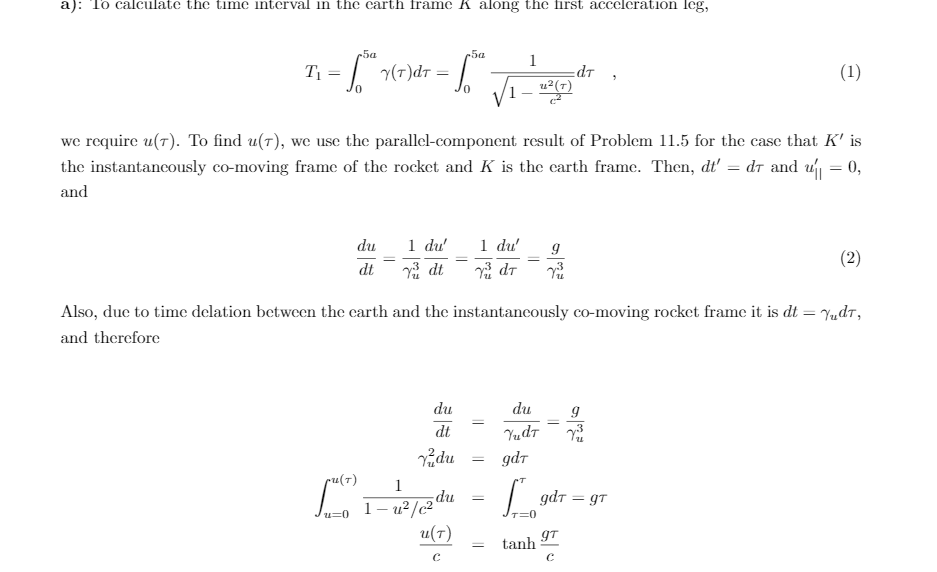
\includegraphics[scale=.7]{FOTOS/hoja 1_1.png}
    \label{fig:hoja1_1}
\end{figure}


